\documentclass[titlepage, a4paper]{article}
\usepackage[utf8]{inputenc}
\usepackage{amsmath}
\usepackage{amssymb}
\usepackage{amsthm}
\usepackage{hyperref}
\usepackage{cleveref}
\usepackage{geometry}
\usepackage{enumerate}
\usepackage{mathtools}
\usepackage{tikz-cd}
\usepackage{tikz}
\usetikzlibrary{fit,arrows,calc,positioning}
\usepackage[backend = biber]{biblatex}
\addbibresource{references.bib}

\makeatletter
\def\input@path{{../Bewijzen/}}

\makeatother

\author{Lucas Levrouw \and Michaël Maex \and Tomas Reunbrouck \and Supervisor: Gabor Szabo}

\title{Kaplansky's Conjectures and Sofic Groups}

\date{\today}

\newcommand{\N}{\mathbb{N}}
\newcommand{\Z}{\mathbb{Z}}
\newcommand{\Q}{\mathbb{Q}}
\newcommand{\R}{\mathbb{R}}
\newcommand{\C}{\mathbb{C}}
\newcommand{\F}{\mathbb{F}}

\newcommand{\card}[1]{\left| #1 \right|}
\newcommand{\inclusion}[1]{\xhookrightarrow{#1}}
\newcommand{\surjection}[1]{\xtwoheadrightarrow{#1}}
\DeclareMathOperator{\sym}{Sym}
\DeclareMathOperator{\im}{im}



\newtheorem{theorem}{Theorem}
\newtheorem{definition}{Definition}
\newtheorem{lemma}{Lemma}
\newtheorem{conjecture}{Conjecture}
\newtheorem{corollary}{Corollary}
\theoremstyle{remark}
\newtheorem{example}{Example}
\newtheorem{remark}{Remark}

\usepackage{import}
\usepackage{xifthen}
\usepackage{pdfpages}
\usepackage{transparent}

\newcommand{\incfig}[1]{%
    \def\svgwidth{.5\columnwidth}
    \import{../Figuren/}{#1.pdf_tex}
}

\begin{document}
\pagenumbering{Alph}
    \maketitle
\pagenumbering{arabic}
\tableofcontents
\pagebreak

\section{Introduction}\label{sec:intro}

\subsection*{The lay of the land}

This thesis discusses the conjecture of Kaplansky which states that any group ring $K[G]$ with $K$ a field is directly finite. That is, the left-invertibility of elements implies their right-invertibility. For general groups and fields, this conjecture remains unanswered. It has been resolved, however, for specific cases, such as the case in which the group $G$ is sofic (the definition of soficity follows in section 3). Some cases require the assumption of another conjecture. For example, when we talk about finite fields $K$ we have a positive result for Kaplansky’s conjecture assuming that all countable groups are surjunctive (definition in section \ref{sec:surjunctivity}). This assumption is known as the conjecture of Gottschalk and will be discussed in detail.

\subsection*{Historical context}

We can trace the origins of the concepts we shall discuss back to the research by John von Neumann throughout the 20th century. First, he introduced the notion of amenable groups in the context of the Banach-Tarski Paradox. It was meant as a generalisation of commutative groups on the one hand and various versions of finite groups on the other. Secondly, he lay the foundations of the study of so-called ‘cellular automata’. What a cellular automaton is, can be explained the following way. Take a set $A$ (finite or infinite), of which we call the elements ‘states’, and a ‘universe’ of ‘cells’, being a group $G$. Now is $A^G$ the set of configurations. The automaton, then, is a map from $A^G$ to itself, satisfying the property that the state of a specific cell in the image is determined by the initial states of the cells in a bounded neighbourhood of this cell.\\
\\
These two concepts may, at first glance, seem completely unrelated. The connection becomes clear, however, when considering the question of surjectivity of these maps on the configuration space. Surjectivity in this context is, intuitively, the property that any configuration can be reached as a result from some other configuration. A configuration that can not be produced because it is not in the image of the (non-surjective) automaton is called a ‘Garden of Eden’. Importantly, such a Garden of Eden always contains a so-called ‘orphan’ which is a finite subset which cannot be produced (a finite Garden of Eden as it were). The Garden of Eden Theorem states that a configuration is a Garden of Eden if and only if it contains such an orphan. From this theorem it follows that the injectivity of the automaton implies its surjectivity. However, the validity of this theorem has only been proven for amenable groups.
Now, groups $G$ for which it is the case that injectivity of an automaton using any finite alphabet implies surjectivity of that automaton are called ‘surjunctive’. We will use the notion of surjunctivity extensively. This, then, brought research eventually to sofic groups, as this is the largest known class of groups of which all members are surjunctive.  

\subsection*{Goal of this paper}

We shall mainly focus on the following two concepts: soficity and surjunctivity. First we shall discuss what it means for a group to be sofic. It is a very broad concept. In fact, there exist no known examples of non-sofic groups \cite{weiss_2000}. This will be illustrated by proving soficity for a few large classes of groups. Furthermore, we shall discuss its connections to other important concepts and group properties such as amenability. Secondly, this paper will cover surjunctivity which is related to soficity but will be used to discuss the connection between the conjectures of Kaplansky and Gottschalk. Specifically, it is known that all sofic groups are surjunctive as well.

\begin{figure}[h]
	\centering
\begin{tikzcd}
	\text{Residually Finite} \arrow[dr, Rightarrow] \\
	& \text{Sofic} \arrow[r, Rightarrow] & \text{Surjunctive} \arrow[r, Rightarrow] & \text{Directly finite}\\
\text{Amenable} \arrow[ur, Rightarrow]
\end{tikzcd}
\caption{A dependency graph of the relevant theorems/properties. }
\end{figure}
\section{Group rings}\label{sec:group_rings}

The setting of Kaplansky's direct finiteness conjecture is about so-called group rings. These are defined as follows


\begin{definition}\label{def:group_ring}
	Let $K$ be a field and $G$ be a group. The \textbf{group ring} $K[G]$ is the set of formal linear combinations
    \[
        \sum_{g \in G} \lambda_g g,
    \]
    where only finitely many $\lambda_g \neq 0$ with operations $+$ and $\cdot$ defined by
    \begin{align*}
        \sum_{g \in G} \lambda_g g + \sum_{g \in G} \mu_g g
        &= \sum_{g \in G} (\lambda_g+\mu_g) g \\
        \left(\sum_{g \in G} \lambda_g g \right) \cdot \left(\sum_{g \in G} \mu_g g \right)
        &= \sum_{g \in G} \left( \sum_{h \in G} \lambda_{h} \mu_{h^{-1}g} \right) g.
        %\sum_{g \in G} \left( \sum_{\substack{g_1, g_2 \in G \\ g_1 g_2 = g}} \lambda_{g_1} \mu_{g_2} \right) g.
    \end{align*}
\end{definition}


\begin{theorem}
    Let $K$ be a field and $G$ a group. Then $K[G]$ is a unital ring.
\end{theorem}


\begin{proof}
    We need to prove associativity of $+$, commutativity of $+$, existence of zero element, existence of additive inverses, associativity for $\cdot$, left distributivity, right distributivity and existence of a unit element.
    % further proof needed
    \begin{description}
    \item[associativity of $+$]
    \begin{align*}
    \left(\sum_{g \in G} \lambda_g g + \sum_{g \in G} \mu_g g\right)+ \sum_{g \in G} \nu_g g
    &= \sum_{g \in G} \left((\lambda_g g + \mu_g g)+\nu_g g\right) \\
    &= \sum_{g \in G} \left(\lambda_g g + (\mu_g g+\nu_g g)\right) \\
    &= \sum_{g \in G} \lambda_g g + \left(\sum_{g \in G} \mu_g g + \sum_{g \in G} \nu_g g \right)
    \end{align*}

    \item[commutativity of $+$]
    \begin{align*}
    \sum_{g \in G} \lambda_g g + \sum_{g \in G} \mu_g g
    &= \sum_{g \in G} (\lambda_g g + \mu_g g) \\
    &= \sum_{g \in G} (\mu_g g + \lambda_g g) \\
    &= \sum_{g \in G} \mu_g g + \sum_{g \in G} \lambda_g g 
    \end{align*}

    \item[existence of $0$]
    \begin{align*}
    \sum_{g \in G} \lambda_g g + \sum_{g \in G} 0 g
    &= \sum_{g \in G} (\lambda_g + 0)g \\
    &= \sum_{g \in G} \lambda_g g
    \end{align*}

    \item[existence of additive inverse]
    \begin{align*}
    \sum_{g \in G} \lambda_g g + \sum_{g \in G} (-\lambda_g g)
    &= \sum_{g \in G} (\lambda_g - \lambda_g) g \\
    &= 0
    \end{align*}

    \item[associativity of $\cdot$]
    \begin{align*}
    \left[\left(\sum_{g \in G} \lambda_g g \right) \cdot \left(\sum_{g \in G} \mu_g g \right)\right ] \cdot \sum_{g \in G} \nu_g g
    &= \left(\sum_{g \in G} \left( \sum_{h \in G} \lambda_{h} \mu_{h^{-1}g} \right) g \right) \cdot \sum_{g \in G} \nu_g g\\
    &= \sum_{g \in G} \sum_{x \in G} \left( \sum_{h \in G} \lambda_{h} \mu_{h^{-1}x} \right) \nu_{x^{-1}g} \,g \\
    &= \sum_{g \in G} \sum_{y \in G} \sum_{h \in G} \lambda_{h} \mu_{y} \nu_{y^{-1} h^{-1}g} \, g \\
    &= \sum_{g \in G} \sum_{h \in G} \lambda_h \left(\sum_{y \in G}\mu_{y} \nu_{y^{-1} (h^{-1}g)}\right)g \\
    &= \left(\sum_{g \in G} \lambda_g g \right) \cdot \left[ \left(\sum_{g \in G} \mu_g g \right) \cdot \sum_{g \in G} \nu_g g \right]
    \end{align*}

    \item[left distributivity]
    \begin{align*}
    \sum_{g \in G} \lambda_g g \cdot \left(\sum_{g \in G} \mu_g g + \sum_{g \in G} \nu_g g \right) 
    &= \sum_{g \in G} \lambda_g g \cdot \sum_{g \in G} (\mu_g + \nu_g) g \\
    &= \sum_{g \in G} \sum_{h \in G} \lambda_h (\mu_{h^{-1}g} + \nu_{h^{-1}g}) g \\
    &= \sum_{g \in G} \left(\sum_{h \in G} \lambda_h \mu_{h^{-1}g} + \lambda_h \nu_{h^{-1}g}\right) g \\
    &= \sum_{g \in G} \lambda_g g \cdot \sum_{g \in G} \mu_g g
        + \sum_{g \in G} \lambda_g g \cdot \sum_{g \in G} \nu_g g
    \end{align*}

    \item[right distributivity]
    \begin{align*}
    \left(\sum_{g \in G} \lambda_g + \sum_{g \in G} \mu_g g\right) \cdot \sum_{g \in G} \nu_g g
    &= \left(\sum_{g \in G} (\lambda_g g + \mu_g) g\right) \cdot \sum_{g \in G} \nu_g g\\
    &= \sum_{g \in G} \sum_{h \in G} (\lambda_h + \mu_h) \nu_{h^{-1}g} g \\
    &= \sum_{g \in G} \sum_{h \in G} \lambda_h \nu_{h^{-1}g} g + \mu_h \nu_{h^{-1}g} g \\
    &= \sum_{g \in G} \lambda_g g \cdot \sum_{g \in G} \nu_g g + \sum_{g \in G} \mu_g g \cdot \sum_{g \in G} \nu_g 
    \end{align*}

    \item[existence of 1]
    \begin{align*}
    \sum_{g \in G} \delta_{g,e} g \cdot \sum_{g \in G} \lambda_g g
    &= \sum_{g \in G} \left(\sum_{h \in H} \delta_{h,e} \lambda_{h^{-1}g} \right) \\
    &= \sum_{g \in G} \lambda_{e^{-1}g} g = \sum_{g \in G} \lambda_g g.
    \end{align*}
    
    \end{description}
\end{proof}

\begin{remark}
	A group ring in general is not commutative. In fact $\mathbb{K}[G]$ is commutative if and only if $G$ is a commutative group. So we will have to be careful when dealing with these rings. 
\end{remark}
We can now state Kaplansky's conjecture.

\begin{conjecture}[Kaplansky]
    Let $K$ be a field and $G$ a group. Then $K[G]$ is directly finite i.e. for all $a, b \in K[G]$, the equation $ab=1$ implies $ba=1$.
\end{conjecture}

To put it shortly, Kaplansky's conjecture states that for all elements in the group ring, left-invertible implies right-invertible. If $K$ is a finite field and $G$ is a finite group, it can quite easily be proven that $K[G]$ is directly finite.

\begin{theorem}
    Let $K$ be a field and $G$ be a finite group. Then $K[G]$ is directly finite.
\end{theorem}
\begin{proof}
    Let $a, b \in K[G]$ and suppose $ab=1$. Now consider the map
    \[
        \phi: K[G] \to K[G]: x \mapsto x a
    \]
    This map is injective. To see this, let $x, y \in K[G]$ such that $xa=ya$. Multiply on the right with $b$ and use the associativity to conclude $x=y$.
    But since $K[G]$ is a finite set, the map must also be surjective. Therefore there exists an $x \in K[G]$ such that $x a = 1$. Furthermore, $x = xab = b$. So we have $b=a$.
\end{proof}

Note how the argument hinges on the fact that the map $\phi$ is guarantied to be surjective by the finiteness of $K$ and $G$. In what follows we will define several ``finiteness'' properties of groups and try to generalise the proof above under weaker assumptions.

\section{Sofic groups}\label{sec:sofic_group}

\subsection{Definition and examples}

    A key notion of interest will be that of a sofic group. We call a group sofic if it can be ``well approximated by a finite permutation group". This is made precise in the following definition.

    \begin{definition}\label{def:Sofic}
	    Let $G$ be a countable group. We say that $G$ is \textbf{sofic} if there exists a sequence $(d_i)_{i \in \N} \in \N ^{\N}$ with associated maps $\Phi_i : G \to \sym(d_i)$ such that $\forall\ g, h \in G$:
        \begin{enumerate}[(i)]
            \item $\displaystyle \lim_{i\to \infty} \frac{1}{d_i} \card{\big\{k \in \{1, \dots, d_i\} \mid (\Phi_i(g) \circ \Phi_i(h))(k) = \Phi_i(gh) (k) \big\}} = 1$
            \item $\displaystyle \lim_{i\to \infty} \frac{1}{d_i}  \card{\big\{k \in \{1, \dots, d_i\} \mid \Phi_i(g)(k) = k \big\}} = \delta_{e,g}$,
        \end{enumerate}
        where $\delta_{e,g}$ is $1$ if $g = e$ and $0$ otherwise.
    \end{definition}

    We will call such a family of maps $\left(\Phi_i : G \to \sym(d_i) \right)_{i \in \N}$ a \emph{sofic approximation} for $G$. It is unkown if every group is sofic.


    % Alternative definitions here (Capraro-Lupini definition, example 2.1.8)

	\subsubsection{Alternative definition}
	There are multiple different definitions of soficity. 
	We will give another definition that we found very enlightening (adapted from definition section 2.1 in \cite{capraro_lupini_2015}.)
	Here soficity is defined based on the concept of a length function.
	\begin{definition}
		On a group $G$ a \textbf{length function} is a map $l: G \to [0,1]$ that maps that satifies for every  $x, y \in G$
		\begin{description}
			\item[triangle inequality] $l(xy) \le l(x) + l(y)$
			\item[symmetry]  $l(x^{-1}) = l(x)$
			\item[positive definite] $l(x) = 0 \iff x =1$
		\end{description}
		A length function is said to be \textbf{invariant} if it is unchanged by conjugation. Meaning that \[
			l(y^{-1}xy) = l(x)
		.\] 
	\end{definition}
	\begin{remark}
		A length is invariant if and only if for every $x, y \in G$ \[
			l(xy) = l(yx)
		.\] 
	\end{remark}
	
	With a invariant length we can define a metric on $G$
	 \begin{definition}
	 Given a group $G$ with a length function $l$ we define the metric \[d: G\times G \to [0,1]: (x,y) \mapsto d(x,y) = l(x,y). \]
	\end{definition}
	\begin{remark}
		This metric is left and right translation invariant. Try to see why.
	\end{remark}
	\begin{remark}
		Given a left and right translation invariant metric $d$ on a group  $G$, we can construct a lenght  $l$ as  \[
			l(x) = d(x, 1)
		.\] 
		It turns out that this gives defines a bijective correspondence between invariant lengts and translation invarant metrics. 
	\end{remark}
	
	Now we will define the length and corresponding metric that we need to define soficity.

	\begin{definition}
		Let $S_n$ be the permutation group on of $\left\{ 1,2,\ldots,n \right\} $. 
		We define the \textbf{Hamming invariant length function} $l_{S_n}$ on $S_n$ to be \[
			l_{S_n}(\sigma) = \frac{1}{n} \card{\left\{ i \in \left\{ 1, \ldots, n \right\} \mid \sigma(i)\ne i \right\} }
		.\] 
		The associated metric is denoted by $d_{S_n}$
	\end{definition}
	We are now able to state an alternative definition of sofic groups.
	\begin{definition} % shouldn't we call this a theorem?
		A countable group $G$ is called sofic, if for every $\epsilon > 0$ and for every finite subset  $F \subset G\setminus\{1\}$ there is $n \in \N$ with and a function to the symmetric group $\Phi: G \to S_n$ such that $\Phi(1) = 1$ and for every  $g, h \in G\setminus \{1\} $:
		\begin{itemize}
			\item $d_{S_n}\left( \Phi(gh), \Phi(g) \circ \Phi(h) \right) < \epsilon$
			\item $l_{S_n} \left( \Phi(g) \right) > 1-\epsilon$
		\end{itemize}
	\end{definition}

    \begin{proof}
    We first prove that this criterion implies our original definition. Since $G$ is countable, we can write $G = \{g_1, g_2, \dots\}$. Now let $i \in \N$ be arbitrary and let $F_i = \{ g_1, g_2, \dots, g_i\}$. Then there exists an $n$ and a function $\Phi_i: G \to S_{n_i}$ such that
    \[
        \begin{cases}
        \forall g, h \in F: d_{S_{n_i}}(\Phi_i(gh), \Phi(g) \circ \Phi(h)) < \frac 1 i \\
        \forall g \in F: \left|\ell_{S_{n_i}}(\Phi_i(g)) - (1 - \delta_{ge}) \right|< \frac 1 i
        \end{cases}
   \]
   Now we clearly have for all $g,h \in G$ that $\lim_{i \to \infty} d_{S_{n_i}}(\Phi_i(gh), \Phi(h)^{-1} \Phi(g)^{-1}) = 0$ and $\lim_{i \to \infty} \ell_{S_{n_i}}(\Phi(g)) = 1 - \delta_{ge}$,  and this is precisely the soficity condition in our first definition.

   Conversely, let $\left(\Phi_i: G \to S_{n_i} \right)_{i \in I}$ be a sofic approximation for $G$. Assume without loss of generality that $\Phi_i(e) = id_{S_{n_i}}$. Now let $\epsilon > 0$ be arbitrary and let $F$ be a finite subset of $G$.
   For all $g,h$ there exists an $i_{g,h} \in \N$ such that for all $i \geq i_{g,h},$
   \[
   d_{S_{n_i}}(\Phi_i(g) \circ \Phi_i(h), \Phi_i(gh)) < \epsilon,
   \]
   and for every $g \in F$ there exists a $j_g$ such that for all $j \geq j_g$
   \[
        \left| \ell_{S_{n_j}} - (1-\delta_{e,g}) \right| < \epsilon
   \]
   Now let $i = \max_{g,h \in F}(i_{gh})$, $j = \max_{g \in F}(j_g)$ and $k = \max\{i,j\}$.
   Then for all $g,h \in G$, we have
   $ d_{S_{n_k}}(\Phi_i(g) \circ \Phi_k(h), \Phi_k(gh)) < \epsilon$ and $\left| \ell_{S_{n_k}} (\Phi_k(g) - (1- \delta_{eg})) \right| < \epsilon$.

    \end{proof}

	This definition is particularly nice because it really makes clear in what sense a soficity means that a group can be approximated by a sequence of symmetric groups. 
	Namely $\Phi$ is an almost morphism in the sense that is maps the product of two elements very close the product of the images. In fact, later in the same section of \cite{capraro_lupini_2015} Lupini goes on by defining the concept of an $(F, \epsilon)$-approximate morphism. 
	\begin{definition}
		Let $G, H$ be groups with invariant length functions. 
		Let $F$ be a subset of $G$ and  $e > 0$.  
		A function $\Phi:  G \to H$ is an $(F,\epsilon)$-approximate morphisms if $\Phi(1) = 1$ and for every $g, h \in F$ 
		\begin{itemize}
			\item $d_H(\Phi(gh),\Phi(g)\circ \Phi(h)) < \epsilon$
			\item $l_H(\Phi(p)) - l_G(g) < \epsilon$
		\end{itemize}
	\end{definition}
	With this language we can say that a group $G$ is sofic if and only if for every $\epsilon >0$ and finite subset $F \subset G$ there exists a $(F,\epsilon)$-approximate morphism to $S_n$ for some  $n$.


	\subsubsection{Examples}
    \begin{example}\label{ex:finite_group_sofic}
    Consider a finite group $G$. Look at the map $\phi: G \to \sym(G): g \mapsto \sigma_g$, where $\sigma_g$ is defined by $\sigma_g(h) = gh$. Clearly, $\phi$ is a homomorphism. Now we can choose $d_i = \card G$ and $\Phi_i = \phi$ for all $i \in \N$. Here we have identified $\sym(G)$ with $\sym(d_i)$. The first condition is satisfied since $\phi$ is a morphism. The second condition follows from the fact that $\sigma_g(h) = gh = h$ if and only if $g$ is the identity.
     Hence every finite group is sofic.
    \end{example}

    % Example: Z

	\begin{example}\label{ex:Z}
	Consider the group $\Z$. Take the sequence of maps $\Phi_{i}: G \to \sym(i): g \mapsto \Phi_{i}(g)$ where $\Phi_{i}(g)$ is defined as the map such that for any $k \in \{1,...,i\}$ : $ \Phi_{i}(g)(k) = (k+g) \mod(i)$. The first condition of soficity is satisfied as for any $i \in N, g,h \in \Z, k \in \{1,..., i\}$ it can be said that 
	\begin{align*}
	(\Phi_{i}(g) \circ \Phi_{i}(h))(k) &= \Phi_{i}(g)((k+h)\mod(i))\\
	&= (k+h+g)\mod(i)\\
	&= (k+g+h)\mod(i)\\
	&= \Phi_{i}(g+h)(k)
\end{align*}		
	Now for the second condition. It is clear that for any $i \in \N, k \in \{1,..., i\}$ : $\Phi_{i}(0)(k) = k$. Now take any $g \neq 0$ and consider $\Phi_{i}(g)$. For any $k \in \{1,...,i\}$ it is perfectly possible that $\Phi_{i}(g)(k) = k$. However this is not the case as soon as $i > |g|$. Then, namely, we have that $|(k+g)-k| < i$ which means that is is not possible that $(k+g)mod(i) = (k)mod(i)$. Thus we have that $(k+g)mod(i) \neq k$ as $(k)mod(i) = k$ for $k<i$ and the inequality is obvious for $k \geq i$.
	\end{example}
    % Example: Direct product of sofic groups is sofic. 

    \begin{example}\label{ex:direct_product_sofic}
        The direct product of two sofic groups is again sofic. Consider two sofic groups $G$ and $H$. Let $(\phi_i: G \to \sym(d_i))_{i \in \N}$ and $(\psi_i: G \to \sym(e_i))_{i \in \N}$ be sofic approximations for $G$ resp. $H$. Now consider $\Phi_i : G \times H \to \sym(d_i+e_i)$ for every $i \in \N$, where $\Phi_i(g, h) \in \sym(d_i+e_i)$ is defined by
        \[
            \Phi_i(g,h)(k) = \begin{cases} \phi_i(g)(k) & \text{if } 1 \leq k \leq d_i \\
            \psi_i(h)(k)+d_i & \text{if } d_i + 1 \leq k \leq e_i
            \end{cases}.
        \]
        It is not hard to show that $(\Phi_i)_{i \in \N}$ is a sofic approximation for $G \times H$. % Write out proof
        Hence finite direct products conserve the soficity property.
    \end{example}


    \section{Properties that Imply Soficity}


    Often, it will be more convenient to check a property that implies soficity than checking it directly as we have done in the examples above. We will discuss two such properties: amenability and residually finiteness.

    \subsection{Amenability}

    Amenable groups are a large class of groups. 
    Many equivalent definitions exists. 
    An extensive study of amenable groups goes beyond the scope of this project. Hence we will not give multiple definitions and prove equivalence nor will we provide proofs for every property of amenable groups.

    For our purposes we will only define amenability for countable groups and take the Følner criterion as definition.

    \begin{definition}\cite{noauthor_folner_2019} \label{def:folner}
	    Let $G$ be a countable group. We say that $G$ satisfies the \textbf{Følner criterion} if there exists a sequence of finite subsets (not necessarily subgroups) $F_1, F_2, \dots \subset G$ such that 
        \begin{enumerate}
            \item for every $g \in G$ there exists an $N \in \N$ such that for all $n > N: x \in F_n$
            \item for all $g \in G$ 
            \[\lim_{i\to \infty} \frac{\card{gF_i \triangle F_i}}{\card{F_i}} = 0, \]
            where $\triangle$ denotes the symmetric difference.
        \end{enumerate}
    \end{definition}
    \Cref{fig:folner} gives a visual intuition for this notion. 
\begin{figure}[ht]
    \centering
    \incfig{folner}
    \caption{An illustration of the Folner criterion. The limit means that the gray part will become very small compared to  $F_n$ itself as $n$ gets large.}
    \label{fig:folner}
\end{figure}
% example: finite group
If a countable group statisfies the Følner condition, we will also call the group \emph{amenable}.\footnote{One can also define amenability also for uncountable groups. In that case however, it is defined differently and the Følner criterion is not equivalent the amenability.}
\subsubsection{Examples}
\begin{example}\label{ex:finite_group_folner}
    Every finite group trivially satisfies the Følner condition. Indeed, we can take $F_i = G$ for every $i \in \N$. Then the first condition is automatically statisfied and we also have $gG \triangle G = G \triangle G = \emptyset$. Hence $\card{gF_i\triangle F_i} = 0$, for all $i \in \N$.
\end{example}

\begin{example}\label{ex:integers_folner}
    The group of integers $\Z$ is also amenable. Let $F_i = \{-i, -i+1, \dots, i-1, i\}$ for every $i \in \N$. The first condition is satisfied. For the second condition, let $k$ be an arbitrary integer. Then
    \[
        \frac{\card{(k + F_i) \triangle F_i}}{\card{F_i}}
        = \frac{\card{\{k-i, k-i+1, \dots, k+i-1, k+i\}\triangle \{-i, -i+1, \dots, i-1, i\}}}{2i+1}
        \leq \frac{2k}{2i+1},
    \]
    and this converges to zero as $i \to \infty$.
\end{example}

\begin{example}
	Counter examples are at least as insightful as examples. 
	The free group $F_n = \left<x_1, x_2, \ldots, x_n \right>, n \ge 2$ is not amenable. 
	To prove this we will have to show that there does not exist a Folner sequence.
	We will prove that for every non-empty finite subset $H \subset F$ the is holds that \[
		\card{\bigcup_{i = 1}^{n} x_iH \cup x_i^{-1}H} \ge (2n-1) \card{H}
	.\] 
	We can prove this using induction on the size of $H$. 
	\begin{description}
		\item[$\card{H} = 1$:] Then $H = \{g\}$. 
			Hence the left hand side set is $\{x_1g, x_1^{-1}, x_2g, x_2^{-1}g, \ldots, x_ng, x_n^{-1}g\} $, which has cardinality $2n$. 
		\item[$\card{H} > 1$:] 
			Let $ h \in H$ be the element that has the most letters in reduced form.
			Consider the set $H' = H\setminus \{h\} $. 
			By the induction hypothesis it holds that
			\[	
				\card{\bigcup_{i = 1}^{n} x_iH' \cup x_i^{-1}H'} \ge (2n-1) \card{H'}
			.\] 
			For atleast $2n-1$ elements of $\{x_1,x_1^{-1},x_2,x_2^{-1},\ldots, x_n, x_n^{-1}\} $ the words $x_ih$ or  $x_i^{-1}h$ have more letters in reduced form than $h$. Let $\Delta = \{ h_1, h_2, \ldots, h_n\} $ be that set.  
			As multiplying by one generator changes the number of letters by $\pm 1$, we see that elements of $\Delta$ are not of the form $x_ih'$ of $x_i^{-1}h'$ for some generator $x_i$ and $h' \in H$. 
			Hence \[
				\card{\bigcup_{i = 1}^{n} x_iH \cup x_i^{-1}H}  \ge \card{\bigcup_{i = 1}^{n} x_iH' \cup x_i^{-1}H'} + 2n-1
 			.\]
			So \[
				\card{\bigcup_{i = 1}^{n} x_iH \cup x_i^{-1}H} \ge (2n-1)\card{H'} + (2n-1) = (2n-1 ) \card{H}
			.\]
	\end{description}
	This clearly contradicts \cref{lem:folner_finite_subset}. 
	We conclude that the free group is not amenable. 
\end{example}
% example: finitely generated groups are not amenable

\subsubsection{Properties of Amenable Groups}

To prove that each group that satisfies the Følner criterion is sofic, we first need the following set-theoretic lemma.

\begin{lemma}\label{lem:finite_bijections} 
        Let $A$ and $B$ be finite sets such that $|A| = |B|$. Given $A' \subset A, B' \subset B$ and a bijection $f': A' \to B'$ there exists a bijection $f: A \to B$ such that $f|_{A'} = f'$. 
    \end{lemma}
    \begin{proof}
        Since $\card A = \card B$ and $\card A' = \card B'$
        \[
        \card{A \setminus A'} = \card A - \card A' = \card B - \card B' = \card{B \setminus B'}.
        \]
        Therefore there exists a bijection $g: A \setminus A' \to B \setminus B'$. Define $f: A  \to B$ by $f(x) = f'(x)$ for all $x \in A'$ and $f(x)=g(x)$ for all $x \in A \setminus A'$. Then $f$ is a bijection and $f|_{A'} = f'$.
    \end{proof}

We now state the proof.

 	\begin{theorem}\label{thm:folner_sofic}
        Every group $G$ that satisfies the Følner criterion is sofic.
    \end{theorem}
    \begin{proof}
        Let $F_1, F_2, F_3, \dots $ be a Følner sequence of $G$.
%Notice that $G = \bigcup_{i \in \N} F_i$ by the first property. So $G$ is countable. 
Choose for every $i \in \N: d_i = |F_i|$. We will implicitly identify $\sym(F_i)$ with $\sym(d_i)$. Now choose maps $\Phi_i: F_i \to \sym(F_i)$ such that $\Phi_i(g)(h) = gh$ whenever $gh \in F_i$, which is possible due to \cref{lem:finite_bijections}. 

We first prove the second condition.
Fix $g, h \in G$. By the Følner criterion we know that 
\begin{align*}
    \lim_{i\to \infty} \frac{\card{g^{-1}F_i \triangle F_i}}{\card{F_i}} &= 0\\
    &= \lim_{i\to \infty} \frac{\card{g^{-1}F_i \setminus F_i} + \card{F_i \setminus g^{-1}F_i}}{d_i}\\
    &= \lim_{i\to \infty} \frac{2\card{ F_i \setminus g^{-1}F_i }}{d_i}\\
    &= \lim_{i\to \infty} \frac{2\card{\left\{ x \in F_i \mid gx \notin F_i \right\}}}{d_i}. 
\end{align*}
This implies that \begin{equation*}
    \lim_{i\to \infty} \frac{\card{\left\{ x \in F_i \mid gx \in F_i \right\}}}{d_i} = 1,
\end{equation*}
or equivalently 
\begin{equation*}%\label{eq:proof_folner1}
    \lim_{i\to \infty} \frac{\card{\left\{ x \in F_i \mid gx \notin F_i \right\}}}{d_i} = 0
\end{equation*}
As $\Phi_i(g)(x) = gx$ whenever $gx \in F_i$, we can see as well that 
$$\lim_{i\to \infty} \frac{\left|\left\{ x \in F_i \mid \Phi(g)(x)\ne gx \right\}\right|}{d_i} = 0.$$
Which proves the second condition for soficity. 

To prove the first condition, we can apply \cref{lem:folner_finite_subset}, which gives that \[
	\lim_{i \to \infty} \frac{\card{\{g,h, gh\} F_i \triangle F_i}}{d_i} = 0
.\]
Which means that 
$$\lim_{i\to \infty} \frac{\left|\left\{ x \in F_i \mid gx,hx,ghx \in F_i \right\}\right|}{d_i}= 1.$$
As $\Phi_i(g)(x) = gx$ whenever $gx \in F_i$, we can see as well that
$$\lim_{i\to \infty} \frac{\left|\left\{ x \in F_i \mid (\Phi(g) \circ\Phi(h))(x) = \Phi(gh)(x) \in F_i \right\}\right|}{d_i}= 1.$$
This proves the first condition for soficity and concludes the proof. 

 	\end{proof}

    \begin{theorem}\label{thm:countable_abelian_folner}
        Every countable abelian group satisfies the Følner criterion. 
    \end{theorem}
    \begin{proof}
        The group $G$ is countable so we can write $G = \{e, g_1, g_2, g_3, \dots\}$.
Consider the sequence of sets $$F_n = \left\{\prod_{i = 1}^n g_i^{a_i} \mid \card{a_i} \le n\right\}.$$ 
It is clear that this set adheres to the first condition of the folner criterion. 
Fix $g_j \in G$. Take any $n > j$.
Let $$H = \left\{\prod_{i = 1, i \ne j}^n g_i^{a_i} \mid \card{a_i} \le n\right\}.$$
Notice that $\bigcup_{i = -n}^{n} g^{i}H = F_n$.
Define the finite sequence of sets $(B_m)_m$ for $m \in \{-n, \dots, n+1\}$ such that  
$B_m = g^mH \setminus \bigcup_{i=-n}^{m-1}g^iH$.
It should be clear that the elements of $(B_n)$ are pairwise disjoint and that  \[
    \bigcup_{i = -n}^n B_n = F_n 
.\] 
It follows that $\sum_{i=-m}^{m} \card{B_i} = \card{F_n}$. We know that 
\begin{align*}
    \card{gF_n \triangle F_n} &= 2 \card{gF_n \setminus F_n} \\
    &= 2 \card{\bigcup_{i = -n}^n g^{i+1}H \setminus \bigcup_{i = -n}^n g^{i}H}\\
    &=  2 \card{g^{n+1}H \setminus \bigcup_{i = -n}^n g^{i}H}\\
    &= 2 \card{B_{n+1}}
\end{align*}
So to show that the $F_n$ adheres to the second condition of the folner criterion, it is sufficient to show that $\frac{\card{B_{n+1}}}{\card{F_n}} \to 0$ as $n \to \infty$.

We claim that $(\card{B_m})$ is a non-increasing sequence. The following calculation shows this.
\begin{align*}
    \card{B_m} &= \card{g^{m}H \setminus \bigcup_{i=-n}^{m-1}g^iH}\\
    &= \card{g^{m-1}H \setminus \bigcup_{i=-n}^{m-1}g^{i-1}H}\\
    &= \card{g^{m-1}H \setminus \bigcup_{i=-n-1}^{m-2}g^{i}H}\\
    &\le \card{g^{m-1}H \setminus \bigcup_{i=-n}^{m-2}g^{i-1}H} = \card{B_{m-1}}
\end{align*}
So $\card{F_n} = \sum_{i=-n}^{n} \card{B_i} \le (2n+1) \card{B_{n+1}}$, which means that $$\frac{\card{B_{n+1}}}{\card{F_n}} \le \frac{1}{2n+1}.$$
So we find that $\frac{\card{B_{n+1}}}{\card{F_n}} \to 0$ which concludes the proof. 
    \end{proof}
    An immediate corollary is:
    \begin{corollary}
    	Every countable abelian group is sofic.	
    \end{corollary}
    % \begin{lemma}
    %     \label{lem:amenable_short_exact_sequence}
    %     Let $A, B, C$ be groups with morphisms $f:A\to B, g:B\to C$ such that
    %     \[\begin{tikzcd}
    %         A \arrow[r, "f", hook] & B \arrow[r, "g", two heads] & C
    %     \end{tikzcd}\] is a short exact sequence. Then $A$ and $B$ are amenable if and only if $C$ is amenable.
    % \end{lemma}
	The following lemma is a known fact about about ameanable groups, that we will use without proof.
    \begin{lemma}
        \label{lem:amenable_short_exact_sequence}
        Let $A, B, C$ be groups and let $f: A\to B$ be an injective morphism and $g:B\to C$ a surjective morphism such that 
        \[\begin{tikzcd}
            A \arrow[r, "f", hook] & B \arrow[r, "g", two heads] & C
        \end{tikzcd}\]
        is an exact sequence i.e. $\im f = \ker g$. Then $A$ and $B$ are amenable if and only if $C$ is amenable.
    \end{lemma}

    \begin{theorem}
        Every countable solvable group is amenable. 
    \end{theorem}
    \begin{proof}
        Let $G$ be a countable solvable group. Then there exists a finite sequence of subgroups such that 
$$\{e\} = G_0 \triangleleft G_1 \triangleleft G_2 \triangleleft \dots \triangleleft G_n = G,$$ and for every $i, 0\le i<n$, the quotient $\frac{G_{i+1}}{G_i}$ is commutative. 
It is clear that $G_0$ is amenable. We will now use finite induction to show that $G$ is amenable as well. 
Take any $i, 0\le i<n$ and assume that $G_i$ is amenable. Then 
\[\begin{tikzcd}
    G_i \arrow[r, "\id", hook] & G_{i+1} \arrow[r, "\pi", two heads] & \frac{G_{i+1}}{G_i}
    \end{tikzcd}\]
is an exact sequence. Because $\frac{G_{i+1}}{G_i}$ is commutative we know by \cref{thm:countable_abelian_folner} that it is amenable. We assumed that $G_i$ is amenable as well. By \cref{lem:amenable_short_exact_sequence} we find that $G_{i+1}$ is amenable as well. This finishes the induction and thus we can conclude that $G_n = G$ is amenable.

    \end{proof}

\subsection{Residually Finite Groups}

Another property that implies soficity is the following.

\begin{definition}\cite{noauthor_residually_2018} \label{def:res_fin}
	We say that a group $G$ is \textbf{residually finite} if for every $g \in G\backslash\{e\}$ there exists a finite group $H$ and a homomorphisms $f:G \to H$ such that $f(g) \ne e$.
\end{definition}


\subsubsection{Examples}

\begin{example}
	The free group generated by $n$ elements is residually finite. 
	Consider $F_k = \left<x_1, x_2, x_3, \ldots, x_k \right>$.
Let \[
a = x_{i_r}^{\epsilon_r n_r}x_{i_{r-1}}^{\epsilon_{r-1}n_{r-1}}x_{i_{r-2}}^{\epsilon_{r-2}n_{r-2}}x_{i_{r-3}}^{\epsilon_{r-3}n_{r-3}} \ldots x_{i_1}^{\epsilon_1n_1}
,\]
where for every $i$ it holds that $n_i \in \Z_{>0}$ and $\epsilon_i \in \left\{ -1,1 \right\} $, be any non-trivial word in reduced form. 
Our goal is to find a morphism to a finite group that doesn't map $a$ to 1. 
Define the sequence $(N_i)_i$ as $N_i = \sum_{j = 1}^{i} n_j$. 
We'll construct a map from $F_k$ to $S_{N_r + 1}$, which is the symmetric group on $\{0,1, 2, \ldots, N_{r}\} $.
By the universal property of free groups it to define a map itis sufficient to choose for every $m$ the image of $x_m$.
We'll define it as follows
\[
x_m \mapsto \prod_{\substack{j \in \{1,\ldots, r\} \\ m = i_j} } (N_{j-1} N_{j-1}+1 \ldots N_{j})^{\epsilon_i}
,\] 
where the brackets denote cycle notation.

Using this morphism we can let $F_k$ act on the set $\{0,1,\ldots, N_r\} $. 
We will deterimne the position of $0$ after the action of $a$ by keeping track of the position of $0$ after every subsequent  action of  $x_{i_m}^{\epsilon_m n_m}$.

We claim that after acting with $x_{i_{m}}^{\epsilon_{m}n_{m}}x_{i_{m}}^{\epsilon_{m}n_{m}} \ldots x_{i_1}^{\epsilon_1n_1}$ the location of  $0$ is at $N_m$.
We will prove this claim by induction.
If  $m=0$ we essentially act with the trivial element. So $0$ is at position $0$.
 Suppose that $m \ne 0$ to zero and that the action of $x_{i_{m}}^{\epsilon_{m}n_{m}}x_{i_{m}}^{\epsilon_{m}n_{m}} \ldots x_{i_1}^{\epsilon_1n_1}$ maps $0$ to $N_m$. 
 We can act with  $x_{i_{m+1}}^{\epsilon_{m+1}n_{m+1}}$. 
 If we look at the cycles of $x_{i_{m+1}}$ we can see that $N_m$ (the position of  $0$ ) is in the cycle $(N_m \ldots N_{m+1})^{\epsilon_{m+1}}$. As zero is in this cycle can solely focus on what happens within this cycle when dealing with powers of $x_{i_{m+1}}$. 
 Taking the $\epsilon _{m+1} n_{m+1}$-th power means that this becomes the cycle $(N_m \ldots N_{m} + n_{m+1})^{n_{m+1}} = (N_{m+1} N_{m+1}-1 \ldots N_m + 1 N_m)$. 
So we see that $0$ now gets mapped to $N_m$, which proves our claim.

As the action of  $a$ maps $0$ to $N_r \ne 0$, we see that the image of  $a$ in  $S_n$ cannot be trivial. 
We conclude that $F_k$ is residually finite.

\begin{figure}[ht]
	\centering
	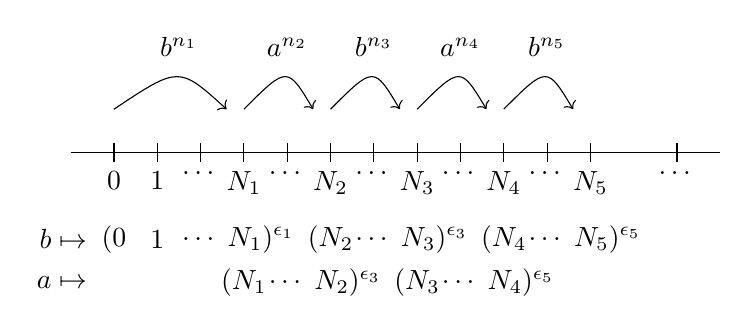
\begin{tikzpicture}[scale = 1.1]
\draw (-.5,0) -- (7,0) ;

\draw[shift={(0,0)},color=black] (0pt,3pt) -- (0pt,-3pt);
\draw[shift={(0,0)},color=black] (0pt,0pt) -- (0pt,-3pt) node[below] 
{$0$};
\draw[shift={(0.5,0)},color=black] (0pt,3pt) -- (0pt,-3pt);
\draw[shift={(0.5,0)},color=black] (0pt,0pt) -- (0pt,-3pt) node[below] 
{$1$};
\draw[shift={(1,0)},color=black] (0pt,3pt) -- (0pt,-3pt);
\draw[shift={(1,0)},color=black] (0pt,0pt) -- (0pt,-3pt) node[below] 
{$\dots$};
\draw[shift={(1.5,0)},color=black] (0pt,3pt) -- (0pt,-3pt);
\draw[shift={(1.5,0)},color=black] (0pt,0pt) -- (0pt,-3pt) node[below] 
{$N_1$};
\draw[shift={(2,0)},color=black] (0pt,3pt) -- (0pt,-3pt);
\draw[shift={(2,0)},color=black] (0pt,0pt) -- (0pt,-3pt) node[below] 
{$\dots$};
\draw[shift={(2.5,0)},color=black] (0pt,3pt) -- (0pt,-3pt);
\draw[shift={(2.5,0)},color=black] (0pt,0pt) -- (0pt,-3pt) node[below] 
{$N_2$};
\draw[shift={(3,0)},color=black] (0pt,3pt) -- (0pt,-3pt);
\draw[shift={(3,0)},color=black] (0pt,0pt) -- (0pt,-3pt) node[below] 
{$\dots$};
\draw[shift={(3.5,0)},color=black] (0pt,3pt) -- (0pt,-3pt);
\draw[shift={(3.5,0)},color=black] (0pt,0pt) -- (0pt,-3pt) node[below] 
{$N_3$};
\draw[shift={(4,0)},color=black] (0pt,3pt) -- (0pt,-3pt);
\draw[shift={(4,0)},color=black] (0pt,0pt) -- (0pt,-3pt) node[below] 
{$\dots$};
\draw[shift={(4.5,0)},color=black] (0pt,3pt) -- (0pt,-3pt);
\draw[shift={(4.5,0)},color=black] (0pt,0pt) -- (0pt,-3pt) node[below] 
{$N_4$};
\draw[shift={(5,0)},color=black] (0pt,3pt) -- (0pt,-3pt);
\draw[shift={(5,0)},color=black] (0pt,0pt) -- (0pt,-3pt) node[below] 
{$\dots$};
\draw[shift={(5.5,0)},color=black] (0pt,3pt) -- (0pt,-3pt);
\draw[shift={(5.5,0)},color=black] (0pt,0pt) -- (0pt,-3pt) node[below] 
{$N_5$};
\draw[shift={(6.5,0)},color=black] (0pt,3pt) -- (0pt,-3pt);
\draw[shift={(6.5,0)},color=black] (0pt,0pt) -- (0pt,-3pt) node[below] 
{$\dots$};

\draw[->] (0, .5) .. controls (.75,1) .. (1.3, .5);
\draw[->] (1.5, .5) .. controls (2,1) .. (2.3, .5);
\draw[->] (2.5, .5) .. controls (3,1) .. (3.3, .5);
\draw[->] (3.5, .5) .. controls (4,1) .. (4.3, .5);
\draw[->] (4.5, .5) .. controls (5,1) .. (5.3, .5);

\node[above] at (.75, 1) {$b^{n_1}$};
\node[above] at (2, 1) {$a^{n_2}$};
\node[above] at (3, 1) {$b^{n_3}$};
\node[above] at (4, 1) {$a^{n_4}$};
\node[above] at (5, 1) {$b^{n_5}$};

\node[left] at (-.2, -1) {$b \mapsto $};
\node[left] at (-.2, -1.5) {$a \mapsto $};

\node at (0, -1) {$(0$};
\node at (0.5, -1) {$1$};
\node at (1, -1) {$\dots$};
\node[right] at (1.2, -1) {$N_1)^{\epsilon_1}$};

\node at (2.5, -1) {$(N_2$};
\node at (3, -1) {$\dots$};
\node[right] at (3.2, -1) {$N_3)^{\epsilon_3}$};

\node at (4.5, -1) {$(N_4$};
\node at (5, -1) {$\dots$};
\node[right] at (5.2, -1) {$N_5)^{\epsilon_5}$};

\node at (1.5, -1.5) {$(N_1$};
\node at (2, -1.5) {$\dots$};
\node[right] at (2.2, -1.5) {$N_2)^{\epsilon_3}$};

\node at (3.5, -1.5) {$(N_3$};
\node at (4, -1.5) {$\dots$};
\node[right] at (4.2, -1.5) {$N_4)^{\epsilon_5}$};

\end{tikzpicture}


<<<<<<< HEAD
	\caption{Illustation of the action in the case of $F_2 = \left<a,b \right>$}
=======
	\caption{Illustration of the action in the case of $F_2 = \left<a,b \right>$}
>>>>>>> ef695785da7d858e253b8e59d8a3e974bffb917b
	\label{fig:}
\end{figure}

\end{example}
% Proof that these are equivalent? Which ones do we actually use?

% example: finite groups

% example: Z

% example: finitely generated groups
\subsection{Properties of Residually Finite Groups}
    \begin{theorem} \label{thm:res_fin_sofic}
        Every countable residually finite group is sofic.
    \end{theorem}
    \begin{proof}
        Let $G$ be a countable residually finite group. As $G$ is countable we can order the elements non-identity elements $g_1, g_2, g_3, \dots$ .
By the first property of residually finiteness, for every $i=1,2,3, \dots$ there exist a group $G_i$ and a homomorphism $f_i: G \to G_i$ such that $f_i(g_i) \ne 1_G$. Consider the direct products $H_n = \prod_{i = 1}^n G_i$ with the induced homomorphisms $h_i: G \to H_i: g \mapsto (f_1(g), f_2(g), \dots, f_i(g))$. Now we will look at the image of $G$ under these morphisms $\Gamma_i = h_i(G)$.


Notice that $\Gamma_i$ is always finite. We will implicitly identify $\sym(\Gamma_i)$ with $\sym(\card{\Gamma_i})$.
For every $i \in \N$, define $d_i = \card{\Gamma_i}$ and $\Phi_i: G \to \sym(\Gamma_i): g \mapsto (a \mapsto ga)$. We claim that this is a sofic approximation sequence for $G$.

For every $k \in \Gamma_i, g, h \in G$ we can see that $(\Phi_i(g) \circ \Phi_i(h))(k) = ghk = \Phi_i(gh)$. So
\[
\{k \in \Gamma_i \mid (\Phi_i(g) \circ \Phi_i(h))(k) = \Phi_i(gh)\} = \Gamma_i.
\]
Then we can see that for all $g,h \in G$:
$$\lim_{i\to \infty} \frac{1}{d_i} \left|\left\{k \in \Gamma_i| (\Phi_i(g) \circ \Phi_i(h))(k) = \Phi_i(gh)\right\}\right| = 1.$$

For every $g \in G, g\ne 1$ there is an $N \in \N$ such that for every $i > N$, $h_i(G) \ne 1_G$. So it is clear that 
$$\lim_{i \to \infty} \frac{1}{d_i} \card{\left\{k \in \Gamma_i \mid \Phi_i(g) = gk \ne k\right\}} = 1.$$
For $g = 1_G$ we find that 
$$\lim_{i \to \infty} \frac{1}{d_i} \card{\left\{k \in \Gamma_i \mid \Phi_i(g) = k \ne k\right\}} = 0,$$
which proves the second condition. 

    \end{proof}

    \subsection{Examples of Sofic Groups}
    \begin{description}
        \item[Finite groups] Every finite group, $G$ satisfies the Følner criterion, as the taking $(G)_n$ as sequence satisfies the properties in \cref{def:folner}.
        \item[Cyclic groups] All finite cyclic groups are taken care of by the previous example. We only need to check $\Z,+$. This group is residually finite as for every $n \in \Z, n \ne 0$ we can consider the natural morphism $\Z \to \Z /(|n|+1)\Z: x \mapsto x \mod |n|+1$. 
        \item[The finite direct product of Sofic groups] Let $G, H$ be sofic groups with sequence $d_i, e_i$ and maps $\sigma_i, \phi_i$ such that the properties of \cref{def:Sofic} hold. It can be (easily) verified that the sequence $(d_i + e_i)_i$ and maps $\psi_i: G \times H \to \sym(d_i + e_i): x (x \le d_i) \mapsto \sigma_i(x), x (x > d_i) \mapsto \phi_i(x -d_i) + d_i$ satisfy \cref{def:Sofic}.
        \item[Finitely generated free groups] They are residually finite.
    \end{description}
    \paragraph{conjectures}
    \begin{itemize}
        \item subgroups of sofic groups
        \item free product of sofic groups
        \item direct product/sum of infinite groups
    \end{itemize}

 

    \section{Surjunctivity}\label{sec:surjunctivity}

    First we define a basic concept in group theory.

    \begin{definition} % van wikipedia gehaald
	    Let $G$ be a group and $X$ be a set. Then $\alpha: G \times X \to X: (g,x) \mapsto \alpha_g(x)$ is called an \textbf{action} of $G$ on $X$ if
        \begin{enumerate}[(i)]
            \item $\forall x \in X: \alpha_e(x) = x$
            \item $\forall g,h \in G, x\in X: \alpha_{gh}(x) = \alpha_g(\alpha_h(x))$.
        \end{enumerate}
    \end{definition}

    In this section we will encounter the set of all maps from $G$ to a finite set $A$. This set will be denoted by $A^G$. We will consider this set as a topological space, the topology on $A^G$ being the product topology, where $A$ carries the discrete topology.

    \begin{definition}
	    Let $G$ be a countable group and $A$ a finite set. Then the \textbf{right shift} $\sigma$ of $G$ on $A$ is defined by
        \[
        \sigma: G \times A^G \to A^G: \left(g, (x_{h})_{h \in G} \right) \mapsto \sigma_g(\omega),
        \]
        where $\sigma_g$ is defined by $\sigma_g\left( (x_{h})_{h \in G} \right) = \left( x_{hg} \right)_{h \in G}$. % Misschien is de ``rij-notatie'' hier niet aangewezen
    \end{definition}

    One can see that $\sigma$ is a $G$-action on $A^G$.
    \begin{definition}
        % Let $G$ be a countable group and $A$ a finite set. 
        % Let $\sigma: G\to \hom{A^{G}}:g \mapsto \left( (x_{h})_{h \in G} \mapsto \left( x_{gh} \right)_{h \in G}  \right)$.
        % The group $G$ is called surjunctive if every injective and continuous $\phi: A^{G}\to A^{G}$ that commutes with $\sigma$ is surjective.
	    Let $G$ be a countable group and $A$ a finite set. The group $G$ is called \textbf{surjunctive} if every injective and continuous $\phi: A^{G}\to A^{G}$ that commutes with $\sigma_g$ for all $g \in G$ is also surjective.
    \end{definition}

    \begin{conjecture}[Gottschalk] \label{conj:gottschalk}
        Every countable group is surjunctive.
    \end{conjecture}
    % \begin{conjecture}[Gottschalk] \label{conj:gottschalk}
    %   Let $G$ be a countable group and $A$ a finite set. 
    %   Let $\sigma: G\to \hom{A^{G}}:g \mapsto \left( (x_{h})_{h \in G} \mapsto \left( x_{gh} \right)_{h \in G}  \right)$.
    %   Then every injective and continuous $\phi: A^{G}\to A^{G}$ that commutes with $\sigma$ is surjective.
    % \end{conjecture}

    It can be proven that every sofic group is surjunctive. However, the proof is not easy. For that reason we will prove it first for the special case of residually finite groups. We will need the following definition

    \begin{definition}
	    Let $G$ be a countable group and $A$ a finite set. Let $H$ be a subgroup of finite index. Then the set of \textbf{$H$-periodic points} is the following subset of $A^G$.
        \[
        P_H = \{ \omega \in A^G  \mid \forall h \in H: \sigma_h\omega = \omega\}
        \]
    \end{definition}

    Since $H$ is of finite index, this set is finite. % more explanation needed
    A key lemma we will further need in our proof of theorem \ref{thm:res_fin_surjunctive} is the following

    \begin{lemma} \label{lem:h-periodic_points}
    The $H$-periodic points are dense in $A^G$, where $A$ is finite set and $G$ is a residually finite countable group.
    \end{lemma}
    \begin{proof}
        Let $f:G \to A \in A^G$. We will prove that there exists a sequence of periodic points that converges to $f$. As $G$ is countable we can lists its elements $G = \{1, g_1, g_2, g_3,\dots\}$. 
        Let $F_n = \{1, g_1, g_2, \dots, g_n\}$. 
        As $G$ is residually finite, for every $g \in F_n^{-1} \cdot F_n,\ g \ne 1$, we can find a map $\pi_g: G \to H_g$, where $H_g$ is a finite group and $\pi_g(g) \ne 1$.  Consider the map \[\pi = \prod_{ \substack{g\in  F_n^{-1} \cdot F_n\\ g\ne 0}} \pi_g
        .\]
        Observe that $\im(\pi)$ is finite, thus $\ker\pi$ is a subgroup of finite index of $G$. 
        For $g_i, g_j \in F, i \ne j$ is is clear that $\pi(g_i) \ne \pi(g_j)$ as $\pi(g_j^{-1} g_i) \ne 1$. 
        This means that there exists a function $\alpha: \im(\pi) \to A$ such that for all $g_i \in F_n: (\alpha \circ \pi)(g_i) = f(g_i)$. 
        Notice that $\alpha \circ \pi \in A^G$. 
        Let $h \in \ker\pi$ and consider the right $h$ shift, $\sigma_h$. 
        Take any $g \in G$. 
        Then 
        \[\sigma_h(\alpha\circ\pi)(g) = (\alpha \circ \pi)(hg) = \alpha(\pi(h)\pi(g)) = \alpha(\pi(g)) = (\alpha\circ\pi)(g).\] Thus $\sigma_g(\alpha \circ \pi) = (\alpha\circ\pi)$.
        So $\alpha\circ\pi$ is a $\ker\pi$ periodic point. 

        For every $F_n =  \{1, g_1, g_2, \dots, g_n\}$ we can construct such a function $\pi_n$ which is an $H$ periodic point and that agrees with $f$ on $F_n$. It is clear that $(\pi_n)_{n\in\N}$ converges to $f$ pointwise as a function. This is sufficient to say that $(\pi_n)_n$ converges to $f$ in the product topology.
    \end{proof}

    Now we can quite easily prove the following result. We follow the proof of Weiss \cite{weiss_2000} here.
    \begin{theorem} \label{thm:res_fin_surjunctive}
    Every residually finite group is surjunctive.
    \end{theorem}
    \begin{proof}
    Let $G$ be a residually finite group and $A$ a finite set. Let $\phi: A^G \to A^G$ be a continuous map which commutes with the right shift $\sigma$. Assume further that $\phi$ is injective. We need to prove that $\phi$ is also surjective. Since $\phi$ commutes with the shift, it follows readily that it maps $H$-periodic points to $H$-periodic points, for any subgroup $H$ of finite index.
Because $P_H$ is finite (for $H$ of finite index), and $\phi$ is injective, the restriction of $\phi$ to $P_H$ is surjective, thus $P_H \subset \phi(A^G)$. Now since $A^G$ is compact, continuous maps from $A^G$ to itself map closed sets to closed sets. Therefore
\[
\phi(A^G) = \overline{\phi(A^G)} \supset
\overline{\bigcup_{\substack{\text{subgroup } H \\ [G : H] < \infty}}\phi( P_H)}
= \overline{\bigcup_{\substack{\text{subgroup } H \\ [G : H] < \infty}} P_H} = A^G,
\]
where we have used lemma \ref{lem:h-periodic_points}. Thus we conclude $\phi$ is surjective.

    \end{proof}

	% Example: Apply this proof to Z
	
\section{Amenable groups are surjunctive}
In this section we present a direct proof of the fact that Amenable groups are surjunctive without using entropy.
\subsection{About Folner Sequences}
We will first need a couple of extra properties about the Folner criterion and Folner sequences.
\begin{lemma}\label{lem:right_folner_sequence}
	If a group $G$ satisfies the folner criterion, then there also exists a folner sequence for the right action of $G$ on itself. 
	I.e. there exists a sequence $F_n$ of finite subsets of $G$ such that 
		\begin{enumerate}
		\item for every $g \in G$ there exists an  $N$ such that for all $n >N$ it holds that $g \in F_n$ 
		\item For every $g \in G$ the folowing is true: \[
				\lim_{n \to \infty} \frac{\card{F_ng \triangle F_n}}{\card{F_n}} = 0
		.\] 
	\end{enumerate}
\end{lemma}
\begin{proof}
	Let $F_n$ be a folner sequence for the left action. 
	It's easy to check that $F_n^{-1}$ will be a Folner sequence for the right action. 
\end{proof}

\begin{lemma}
	Let $F_n$, $E_n$ be two (right) folner sequences for $G$. Then $F_n \cup E_n$ is a (right) Folner sequence for $G$.
\end{lemma}
\begin{proof}
	We'll prove it for odinary (left) Folner sequences as the proof is completely analogous for right Folner sequences.
	The first property is obivously satisfied. 
	Let's have a look at the limit.
	\begin{align*}
		\lim_{n \to \infty} \frac{\card{g(F_n \cup E_n) \triangle (F_n \cup E_n)}}{\card{F_n \cup G_n}} &= 2 \lim_{n \to \infty} \frac{\card{(gF_n \cup gE_n)\setminus (F_n \cup E_n)}}{\card{F_n \cup E_n}} \\
														&= 2 \lim_{n \to \infty} \frac{\card{F_n \setminus (gF_n \cup g E_n) \cup E_n\setminus (gE_n \cup gF_n) }}{\card{F_n \cup E_n}} \\
														&\le 2 \lim_{n \to \infty} \frac{\card{gF_n \setminus F_n} + \card{gE_n \setminus E_n}}{\card{F_n \cup E_n}}\\
														&\le 2 \lim_{n \to \infty}  \frac{\card{gF_n \setminus F_n}}{\card{F_n}} + \frac{\card{gE_n \setminus E_n}}{\card{E_n}} \\
														&=  \lim_{n \to \infty} \frac{\card{gF_n \triangle F_n}}{\card{F_n}} +  \frac{\card{gE_n \triangle E_n}}{\card{E_n}}= 0  
	.\end{align*}
	Hence we see that the claim is valid.
\end{proof}
We find the following corollary. 
\begin{corollary}\label{cor:product_folner_sequence}
	Let $B \subset G$ be a finite subset and $F_n$ be a (left or right) Folner sequence of $G$. Then are $BF_n$ and $F_nB$ again Folner sequences.
\end{corollary}

\begin{lemma}\label{lem:folner_finite_subset}
	Let $F_n$ be a Folner sequence. Then for every finite subgroup $B \subset G$ it holds that  \[
	\lim_{n \to \infty} \frac{\card{BF_n \triangle F_n}}{\card{F_n}} = 0	
	.\] 
\end{lemma}
\begin{proof}
	TODO
\end{proof}
\begin{remark}
	A similar result holds for a right Folner sequence.
\end{remark}
\subsection{About surjunctivity}
In the following section $G$ will be a fixed amenable group, $A$ a fixed finite set and $\phi: A^{G} \to A^{G}$ a fixed continuous injective function that commutes with the right shift. 
We will also denote a fixed element of $A$ with $0$.

\begin{lemma}
	There exists a finite subset $\Gamma \subset G$ such that the value of $\phi((x_g)_g)(1)$ is only dependent on the values of $x_h$ where  $h \in \Gamma$. 
	I.e. if for some  $(x_g)_g, (y_g)_g \in A^{G}$ it holds that $x_g = y_g$ for all $g \in \Gamma$, then $\phi((x_g)_g)(1) = \phi((y_g)_g)(1)$.
\end{lemma}
\begin{proof}
	Choose any $a \in A$. As $\phi$ is continuous we know that \[
	\phi^{-1}\left( \prod_{g\in G} \begin{cases}
			\{a\} & g = 1\\
			A & g \ne 1
	\end{cases} \right)
\]
	is open. Hence is contains a basis open  \[
	U_a=\prod_{g \in G}\begin{cases}
		\{\ldots\} & g \in \Gamma_a\\
		A & g \not\in \Gamma_a
	\end{cases}
	,\] 
	for some finite set $\Gamma_a \in G$. 

	We can create such  $\Gamma_a$ for every $a \in A$. 
	Hence if  
	If we take  $\Gamma = \bigcup_{a \in A} \Gamma_a$, we see that the value of $\phi((x_g)_g)(1)$ is only dependent on the values of  $x_h$ where $h \in \Gamma$. 
\end{proof}
From this point on we will also fix $\Gamma$. 
\begin{corollary}
	For any $k \in G$ the value of $\phi((x_g)_g)(k)$ is only dependent on the values of $x_{kh}$ where $h \in \Gamma$.
\end{corollary}	
\begin{proof}
	As $\phi$ commutes with the right shift  $\sigma_k$ we know that $\sigma_k\phi = \phi\sigma_k$. Applying the previous lemma immediately gives the result.
\end{proof}

\begin{corollary}\label{cor:differ_in_image}
	If $(x_g)_g, (y_g)_g \in A^{G}$ only differ on a set $H \subset G$, ie $\forall g \not\in H:x_g = y_g$,
	then  $\phi((x_g))$ and $\phi((y_g))$ will only differ on $H\Gamma^{-1}$.
\end{corollary}
\begin{proof}
	Take $g \not\in H\Gamma^{-1}$. Then $\phi((x_h)_h)(g)$ and $\phi((x_h)_h)(g)$ will only depend on  $\{x_{g\gamma}\mid \gamma \in \Gamma\}$ and $\{y_{g\gamma}\mid \gamma \in \Gamma\} $. But  $g\Gamma \cap H = \emptyset$. Hence $x_{g\gamma} = y_{g\gamma}$ for all $\gamma \in \Gamma$. By the previous corollary we see that $\phi((x_g)) = \phi((y_g))$.
\end{proof}

\begin{definition}
	We say that $(x_g)_g$ has support $H$ if $x_g = 0$ for all $g \not\in H$.
\end{definition}
Let $A_H$ be the set of all element of  $A^{G}$ with support $H$. We can implicitly identify $A_H$ with $A^{H}$.

\begin{lemma}\label{lem:injective_restriction}
	Let $H$ be any finite subset of $G$. Consider the function  \[
		\psi:A_H \to A ^{H\Gamma^{-1}}: (x_g) \mapsto \left(h \mapsto \phi((x_g)_g)(h)\right)
	.\]  
	This function is an injection. 
\end{lemma}
\begin{proof}
	Suppose that $x= (x_g)_g, y = (y_g)_g \in A^{H}$ have the same image under $\psi$. As $x, y$ can only differ on $ H$ their images under $\phi$ cannot differ in $G\setminus H\Gamma^{-1}$ (see \cref{cor:differ_in_image}). Because they also have the same image under/ $\psi$, we know that $\phi(x)$ and $\phi(y)$ must also agree on $H\Gamma^{-1}$. Hence $\phi(x) = \phi(y)$. By the injectivity of $\phi$ we find that $x = y$.
\end{proof}

At this point we're almost ready to prove that $G$ is surjunctive, i.e.\ $\phi$ is surjective. 
In order to show this will show that for any finite subset $B\subset G$ and a map $f:B \to A$ we can find a $x \in A^{G}$ such that $\phi\left(x \right) |_B  = f$. Then we can finish the proof by showing that they image of $\phi$ is dense and using compactness.

\bigskip

For now, lets fix the set $B$ and the map $f:B \to A$. 

\begin{lemma}\label{lem:copies_of_B}
	Let $F$ be any finite subset of $G$. There exists a subset $F' \subset F$ such that for any two  $s,t \in F', s\ne t$ it holds that $B\cdot s$ and  $B\cdot t$ are disjoint and $\card{F'} \ge \frac{\card{F}}{\card{B}^2} $
\end{lemma}
In other words, the set  $BF$ contains at least $\frac{\card{F}}{\card{B^2}}$ disjoint `copies' of $B$. Here copy of $B$ means $B\cdot x$ for some $x \in G$.
\begin{proof}
We will construct $F'$ in a very adhoc manner. 
Start of with $F' = \emptyset$ and $H = F$. Choose any  $f \in H$. Add $f$ to $F'$. Consider $\{g \in F | B\cdot g \cap B\cdot f \ne \emptyset\} $. This set has atmost $\card{B}^2$ elements. 
We can scrap these elements form $H \leftarrow H \setminus \{g \in F | B\cdot g \cap B\cdot f \ne \emptyset\}$. Now we take a new  $f \in H$ and repeat the process.
We can repeat this atleast $\frac{\card{F}}{\card{B^2}}$ therefore $F'$ contains atleast as many elements. 
By the construction we see as well that for any $s, t \in F', s\ne t$ the the copies  $B\cdot s, B\cdot t$  are disjoint.
\end{proof}

We are finally setup to proof that all amenable groups are surjunctive.
\begin{theorem}
	Let $G$ be a countable amenable group and  $A$ be finite set, where we will choose one element and denote it with $0$. Let  $\phi: A^{G} \to A^{G}$ be a injective, continuous map that commutes with the right shift. Then $\phi$ is surjective.
\end{theorem}

\begin{proof}
	Lets fix a finite subset $B \subset G$ and a map $f:B\to A$. 
	Suppose that there does not exists a  $x \in A^{G}$ such that $\phi(x)|_B = f$.
	Notice that this means that for any copy of $B$, take  $B\cdot s$, the image of $\phi$ does not contains a function  $\phi(x)$ such that when restrited to  $B\cdot s$ it is $f': B\cdot s \to A: x \mapsto f\left( x s^{-1} \right) $.

	Let $F_n$ be a right Folner sequence of $G$. By \cref{cor:product_folner_sequence} we know that $BF_n$ is a right Folner sequence as well. 

	Fix  $n$ for a moment. By \cref{lem:injective_restriction} the function \[
		\psi: A^{BF_n} \to A^{BF_n\Gamma^{-1}}: x \mapsto (g \mapsto \phi(x)(g))
	.\] 
	is injective.
	\Cref{lem:copies_of_B} states that we can choose  $ \left\lceil \frac{\card{F_n\Gamma}}{\card{B}^2} \right\rceil $ disjoint copies of $B$ in $BF_n\Gamma$. 
	We know that for every such copy of $B$ the number of possible values at the coordinates of this copy is  $\card{A}^{\card{B}} -1$ by our assumption at the start of this proof.
	Hence there exists a set $\mathcal{A} \subset A^{BF_n\Gamma^{-1}}$ of cardinality \[
		\card{\mathcal{A}} = \card{A}^{\card{BF_n\Gamma^{-1}}- \card{B}\left\lceil \frac{\card{F_n\Gamma^{-1}}}{\card{B}^2} \right\rceil } \cdot (\card{A}^{B} -1)^{\left\lceil \frac{\card{F_n\Gamma^{-1}}}{\card{B}^2} \right\rceil }
\]
such that $\im\psi \subset \mathcal{A}$. 
As $\psi$ is injective it follows that $\card{A^{BF_n}} \le \card{\mathcal{A}}$. Hence
\[
	\card{A}^{\card{BF_n}} \le 
	\card{A}^{\card{BF_n\Gamma^{-1}}- \card{B}\left\lceil \frac{\card{F_n\Gamma^{-1}}}{\card{B}^2} \right\rceil } \cdot (\card{A}^{B} -1)^{\left\lceil \frac{\card{F_n\Gamma^{-1}}}{\card{B}^2} \right\rceil }
.\]
By taking the logarithm of both sides we obtain
\[
	\card{BF_n}\ln(\card{A}) \le \card{BF_n\Gamma^{-1}} \ln(\card{A}) - \left\lceil \frac{\card{F_n\Gamma^{-1}}}{\card{B}^2} \right\rceil \left( \ln(\card{A}^{\card{B}}) - \ln(\card{A}^{\card{B}} -1) \right)   
.\]
By dividing both sides by $\card{BF_n}$ we see 
\[
	\ln(\card{A}) \le \frac{\card{BF_n\Gamma^{-1}}}{\card{BF_n}} \ln(\card{A}) - \frac{1}{\card{BF_n\Gamma^{-1}}}\left\lceil \frac{\card{F_n\Gamma^{-1}}}{\card{B}^2} \right\rceil \left( \ln(\card{A}^{\card{B}}) - \ln(\card{A}^{\card{B}} -1) \right)   
.\]
\Cref{lem:folner_finite_subset} shows that $\lim_{n \to \infty} \frac{\card{BF_n\Gamma}}{\card{BF_n}} = 1$. 
So we know as well that $\lim_{n \to \infty} \frac{1}{\card{BF_n\Gamma}} \left\lceil \frac{\card{F_n\Gamma}}{\card{B}^2} \right\rceil \ge \frac{1}{\card{B}^3} $. 
Therefore \[
	\ln(\card{A}) \le \ln(\card{A}) - \frac{1}{\card{B}^3} \left(\ln(\card{A}^{\card{B}}) - \ln(\card{A}^{B} - 1) \right)
,\]
which is clearly nonsense. 
So our initial assumption is false. 

\bigskip

This means that there exists a $x \in A^{G}$ such that $\phi(x)|_B = f$. As this is true for every  $B$ and $f:B\to A$ we see that the image of  $\phi$ must be dense in $A^{G}$. As a map on compact spaces maps closed sets on closed sets we see that the image of $\phi$ must be $A^{G}$. 
We conclude that $\phi$ is surjective!

\end{proof}

	\section{Kaplansky's direct finiteness condition for finite fields}
	Let us recall the statement of Kaplansky's direct finiteness condition.
	\begin{definition}
		Let $K$ be a field and $G$ be a group. The group ring $K[G]$ is called \textbf{directly finite} if every  $a \in K[G]$, that is left invertible, is right invertible as well. 
		
	\end{definition}
	Kaplansky conjectured that all group rings are directly finite and Weiss showed that this is true for all sofic groups \cite{weiss_2000}. 
	In the case where $R$ is a finite field, Weiss did this by first proving the the surjunctivity of sofic groups.
	He finished the argument by proving that the group rings of finite fields and surjunctive groups are directly finite.  

	In this section we will give the details of a proof of that last step. 
	I.e we'll prove the following theorem. 
	\begin{theorem}\label{thm:gottschalk_kaplansky}
		Let $\F$ be a finite field and $G$ be a surjunctive group. Then $\F[G]$ is directly finite. 
	\end{theorem}
	It looks like we will need to use the surjuctivity on $\F^{G}$. Hence we need some statement that relates $\F^{G}$ to $\F[G]$.
	\begin{lemma}
		For a group $G$ and field $\mathbb K$ we can consider $\mathbb{K}^{G}$ as a left $\mathbb{K}[G]$-module, with pointwise addition and multiplication defined as
		\begin{align*}
			\cdot : (\mathbb{K}[G] , \mathbb{K}^{G}) &\longrightarrow \mathbb{K}^{G} \\
		\left( \sum_{g \in G} a_g g,  (x_g)_{g \in G}\right)  &\longmapsto \left( \sum_{h \in G} a_h x_{h^{-1}g} \right)_{g \in G}
	.\end{align*} 
	\end{lemma}
	\begin{proof}
		We check the module axioms one by one.
		In the following calculations $r = \sum_{g \in G}^{} r_g g,\ s = \sum_{g \in G}^{} s_g g$ are arbitrary elements of $\mathbb{K}[G]$ and $x = (x_g)_{g \in G}, y = (y_g)_{g \in G}$ are arbitrary elements of $\mathbb{K}^{G}$.
		\begin{description}
			\item[left distributivity] 
				\begin{align*}
					r\cdot (x+y) &= \left( \sum_{h \in G} r_h (x_{h^{-1} g} + y_{h^{-1} g}) \right)_{g \in G} \\
						     &= \left( \sum_{h \in G} r_h x_{h^{-1} g} \right)_{g \in G}  + \left( \sum_{h \in G} r_h y_{h^{-1}g} \right)_{g \in G}  \\
						     &= r\cdot x + r\cdot y 
				.\end{align*}
			\item[right distributivity]
				\begin{align*}
					(r + s)\cdot x &= \left( \sum_{h \in G} (r_h + s_h) x_{h^{-1} g} \right)_{g \in G}  \\
						       &= \left( \sum_{h \in G} r_h x_{h^{-1}g} \right)_{g \in G} + \left( \sum_{h \in G} s_{h} x_{h^{-1}g}  \right)_{g \in G} \\ 
						       &= r\cdot x + s \cdot y 
				.\end{align*}
		
			\item[associativity]
				 \begin{align*}
					 (rs)\cdot x &= \left( \sum_{g_1 \in G} \sum_{g_2 \in G} r_{g_1} s_{g_2} g_1 g_2 \right) \cdot (x_{g})_{g \in G} \\
						     &= \left( \sum_{h \in G} \sum_{k \in G} r_{k}s_{k^{-1}h} h\right) \cdot  \left( x_{g} \right)_{g \in G} \\
						     &= \left( \sum_{h \in G} \sum_{k \in G} r_k s_{k^{-1}h} x_{h^{-1}g} \right)_{g \in G}  \\
						     &= \left( \sum_{h \in G} \sum_{k \in G} r_k s_{k^{-1}h} x_{(k^{-1} h)^{-1}(k^{-1}g)} \right)_{g \in G}  \\
						     &= \left(\sum_{h \in G} r_h h\right) \cdot  \left( \sum_{k \in G} s_{k} x_{k^{-1}g} \right)_{g \in G} \\
						     &= r(s\cdot x) 
				.\end{align*}
			\item[unity]
				\begin{align*}
					1\cdot x &= (x_{1^{-1} g})_{g \in G} \\
						 &= x\\
				.\end{align*}
		\end{description}
	\end{proof}
        \begin{remark}
        The way $\F^{G}$ is defined as a $\F[G]$-module is not completely abitrary. It should be easy to see that  $\F^{G}$ can be represented as formal sums $\sum_{g \in G} x_g g$, just like $\F[G]$, but where we now allow infinite sums. 
        The definition of the multiplication between  $\F[G]$ and  $\F^{G}$ agrees with the obvious multiplication with $\F^{G}$ represented as above. 
    \end{remark}
    
	We're now ready to give a proof of \cref{thm:gottschalk_kaplansky}.
	\begin{proof}
		Let $\F$ be a finite field and $G$ be a surjunctive group. 
		Let $a = \sum_{g \in G} a_g g \in \F[G]$ be a left invertible element with left inverse $b$, i.e.  $b a = 1$. 
		Consider the map $\phi: \F^{G} \to \F^{G}: x \mapsto a\cdot x$. Notice that this map 
		\begin{itemize}
			\item is injective. Suppose that $\phi(x) = \phi(y)$. Then $a\cdot x = a\cdot y$. So $ba\cdot x  = x$ and $ba \cdot y = 1\cdot y = y$. Hence $x = y$.
			\item commutes with the bernoulli shift  $\sigma_k$. 
				 \[
					 \sigma_k \phi(x) 
					 = \sigma_k\left( \sum_{h \in G} a_h x_{h^{-1}g} \right)_{g \in G} 
					 = \left( \sum_{h \in G} a_h x_{h^{-1}gk} \right)_{g \in G} 
					 = \left( \sum_{h \in G}a_h h \right) \cdot (x_{gk})_{g \in G} = \phi(\sigma_k(x)) 
				\]
			\item is continuous. 
			One can easily check that the set $\left\{ U_{h, t} \right\}$, where \[
			U_{h,t}:= \prod_{g \in G} \begin{cases}
				\F & h \ne g\\
				\{t\}& h = g
			\end{cases}
			.\] 
			is a subbasis of $\F^{G}$. 
			Hence, to prove that $\phi$ is continuous it is sufficient to check that $\phi^{-1}(U_{h, t})$ is open for every $h \in G, t\in \F$.
			Notice that an  $(x_g)_{g \in G} \in \F^{G}$ is in $\phi^{-1}(U_{h,t})$ if and only if $\sum_{k \in G} a_k x_{k^{-1}h} = t$. 
			Remember that $a_k$ is nonzero only for a finite number subset $X$,  $k\in X \subset G$. 	
			So $\phi^{-1}(U_{h, t})$ is closed under addition with an element of  \[
			\prod_{g \in G} \begin{cases}
				\F & hg^{-1}  \not\in X\\
				\{0\} & hg^{-1} \in X 
			\end{cases}
			.\] 
			Let  $(x_g) \in \phi^{-1}(U_{g,t})$. We see that  \[
				(x_g) \in \prod_{g \in G} \begin{cases}
					\F & hg^{-1} \not\in X\\
					\{x_g\} & hg^{-1} \in X
				\end{cases}
				\subset \phi^{-1}(U_{h, t})
			.\] 
			So $\phi^{-1}(U_{h,t})$ is open. Hence $\phi$ is continuous.			
		\end{itemize}
		By the surjunctivity of $G$ we find that $\phi$ is surjective as well. In particular this means that there exists a $y = (y_g)_{g \in G}$ such that $\phi(y) = (\delta_{g, 1})_{g \in G}$, where $\delta$ is the kronecker delta.
		By multiplying with $b$ on the left we find that \[
			 y = ba\cdot y = b\cdot (\delta_{g, 1})_{g \in G} = \left( \sum_{h \in G} b_{h} \delta_{h^{-1}g, 1} \right)_{g \in G} = \left( \sum_{h \in G} b_{h} \delta_{h, g} \right)_{g \in G}
		 = \left( b_{g} \right) _{g \in G}.\] 
		This means that \[
		a\cdot y = \left( \sum_{h \in G} a_h b_{h^{-1}g} \right)_{g \in G} = \left( \delta_{g, 1} \right) _{g \in G} 
	.\] 
	In other words
	\[
	\sum_{h \in G} a_h b_{h^{-1}g} = \delta_{g, 1}
	.\]
	But this means exactly that $ab = 1$. So  $a$ is right invertible as well. 
	\end{proof}	
	
	
	\pagebreak
	\printbibliography





\end{document}
